\documentclass{beamer}
\usetheme{Warsaw}
\setbeamertemplate{headline}{}

\usepackage{ae,lmodern}
\usepackage[english]{babel}
\usepackage[utf8]{inputenc}
\usepackage[T1]{fontenc}

\usepackage{caption}
\captionsetup[figure]{labelformat=empty}

\PassOptionsToPackage{usenames,dvipsnames}{xcolor}
\usepackage{xcolor,colortbl}
\definecolor{DarkGrey}{HTML}{222222}
\definecolor{DarkBlue}{HTML}{004BA9}
\definecolor{DarkRed}{HTML}{CC1111}
\definecolor{DarkGreen}{HTML}{117711}
\definecolor{DarkOrange}{HTML}{CC7000}
\definecolor{LightGrey}{HTML}{DDDDDD}
\definecolor{LightBlue}{HTML}{F0F8FF}
\definecolor{codegreen}{rgb}{0,0.6,0}
\definecolor{codepurple}{rgb}{0.58,0,0.82}

\usepackage[cache=false]{minted}
\setminted[bash]{
   bgcolor=LightBlue,
   breaklines, breakanywhere,
   frame=single,
   autogobble
}
\usemintedstyle[python]{native}
\setminted[python]{
   bgcolor=black,
   breaklines, breakanywhere,
   autogobble
}

\usepackage{listings}
\usepackage{lstautogobble}
\lstdefinestyle{bash}{
    backgroundcolor=\color{DarkGrey},   
    commentstyle=\color{codegreen},
    keywordstyle=\color{magenta},
    numberstyle=\tiny\color{DarkGrey},
    stringstyle=\color{codepurple},
    basicstyle=\ttfamily\tiny\color{LightGrey},
    escapeinside={\%*}{*)},
    breakatwhitespace=false,         
    breaklines=true,                 
    captionpos=b,                    
    keepspaces=true,                 
    numbers=left,                    
    numbersep=5pt,                  
    showspaces=false,                
    showstringspaces=false,
    showtabs=false,
    showlines=false,
    tabsize=2
}

\usepackage{tikz}
\usetikzlibrary{calc,decorations.pathreplacing,arrows,arrows.meta,shapes,patterns, positioning}
\newcommand\BigLength{14.6em}
\newcommand\Height{2em}
\newcommand\Sep{0.6em}
\newcommand\Center{\BigLength*1/2}
\newcommand\BigBox{\BigLength+\Sep}
\newcommand\HalfBox{\BigLength*1/2-\Sep*1/4}
\newcommand\HalfLength{\BigLength*1/2-\Sep*5/4}
\newcommand\CenterL{\BigLength*1/4-\Sep*1/8}
\newcommand\CenterR{\BigLength*3/4+\Sep*1/8}
\tikzstyle{layer}=[rectangle,thick,text centered,
                     minimum height=\Height,minimum width=\BigLength]
\tikzstyle{short}=[rectangle,thick,text centered,
                     minimum height=\Height,minimum width=\HalfLength]
\tikzstyle{dibox}=[rectangle,thick,semitransparent,
                     minimum height=(\Height+\Sep)*2,minimum width=\BigBox]
\tikzstyle{vmbox}=[rectangle,thick,semitransparent,
                     minimum height=(\Height+\Sep)*3,minimum width=\HalfBox]
\tikzstyle{ctbox}=[rectangle,thick,semitransparent,
                     minimum height=(\Height+\Sep)*2,minimum width=\HalfBox]
\tikzstyle{vebox}=[rectangle,thick,semitransparent,
                     minimum height=(\Height+\Sep)*1,minimum width=\HalfBox]

\usepackage{hyperref}
\usepackage{grffile}


\AtBeginSection[]
{
   \begin{frame}
      \tableofcontents[currentsection]
   \end{frame}
}

\AtBeginSubsection[]
{
   \begin{frame}
      \tableofcontents[currentsection, currentsubsection, sectionstyle=shaded]
   \end{frame}
}

%----------------------------------------------------------------------------------------
\title{Introduction to Data Science}
\subtitle{with Python}
%----------------------------------------------------------------------------------------
\author{Alexis Bogroff}
\date{\today}



\begin{document}

\begin{frame}
   \titlepage
\end{frame}

\begin{frame}\frametitle{Presenter}
   \begin{minipage}{0.3\linewidth}
      \centering
      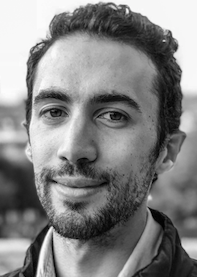
\includegraphics[width=0.6\textwidth]{../images/AlexisBogroff.png} \\
   \end{minipage}
   \begin{minipage}{0.6\linewidth}
      \noindent Alexis Bogroff \\
      Lecturer and Mentor in Data Science \\
      at Paris 1 Panthéon-Sorbonne, ESILV, Openclassrooms, EM-Lyon
   \end{minipage}
   \\[2ex]
   \visible<2->{\begin{itemize}
      \item 4 years Teaching Assistant and lecturer in VBA, Python for finance, SQL, Data Analysis and Data Science
      \item 9 months Researcher Assistant at Paris 1 Panthéon-Sorbonne within H2020 European Project
      \item 1 year Data Scientist at Pléiade Asset Management
   \end{itemize}}
   \hfill
\end{frame}

% \begin{frame}\frametitle{Overview}
%    \Large
%    \centering
%    Financial Engineering with Python Linux and Git \\[2ex]
%    \begin{minipage}{0.32\linewidth}
%       \includegraphics[width=0.8\textwidth]{../images/linux-1-logo-svg-vector.pdf}
%    \end{minipage}
%    \begin{minipage}{0.32\linewidth}
%       \includegraphics[width=0.8\textwidth]{../images/Git-logo.pdf}
%    \end{minipage}
%    \begin{minipage}{0.32\linewidth}
%       \includegraphics[width=0.9\textwidth]{../images/Python_logo_and_wordmark.pdf}
%    \end{minipage}
%    \pause
%    \\[3ex]
%    Free and everywhere stack \\
%    To find a job and be operational
% \end{frame}

% \begin{frame}\frametitle{Lecture Organisation}
%    \begin{itemize}[<+->]
%       \item Prerequisite:
%       \begin{enumerate}
%          \item Have a Linux environment working on your personal computer
%          \item[] (it can be WSL2 on Windows, Amazon EC2 for a distant solution)
%          \item Install Git
%          \item Install Python
%       \end{enumerate}
%       \vspace{2em}
%       \item Exam:
%       \begin{itemize}
%          \item Last QCM 1/2
%          \item Project 1/2
%       \end{itemize}
%    \end{itemize}
% \end{frame}


\begin{frame}
   \tableofcontents
\end{frame}

% =============================================================================
% =============================================================================
\section{Data Analysis}
% 3 Hours course (for Analysis and Pre-processing)
% =============================================================================
% =============================================================================


%------------------------------------------------------------------------------
\subsection{Measures}
%------------------------------------------------------------------------------


\begin{frame}\frametitle{Measures}
   \begin{itemize}
      \item Centrality:
      \begin{itemize}
         \item Goal: representation of the majority's value
         \item Mean (average): average age, mean size
         \item Median: median salary, median patrimony
      \end{itemize}
      \item Dispersion:
      \begin{itemize}
         \item Goal: majority's spread (variation) around the central value
         \item Standard deviation (sqrt variance): financial markets volatility
         \item Interquartile Range (IQR)
         \item Min-Max: job proposal salary
      \end{itemize}
   \end{itemize}
\end{frame}



\subsection{Centrality}
%------------------------------------------------------------------------------

\begin{frame}\frametitle{Pandas - Mean}
   \begin{minipage}{0.58\linewidth}
      \begin{itemize}
         \item Sensible to extreme values
         \begin{itemize}
            \item Age: good representation
            \item Patrimony: biased, not representative
         \end{itemize}
      \end{itemize}
      \vspace{.5cm}
      $$mean = \frac{x_1 + x_2 + ... + x_n}{n}$$
      \begin{figure}[H]
         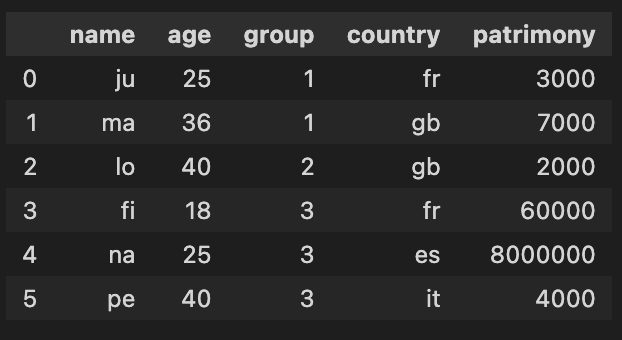
\includegraphics[width=4cm]{../images/illustrations/data_analysis_df_1.png}
      \end{figure}
   \end{minipage}
   \begin{minipage}{0.38\linewidth}
      \begin{figure}[H]
         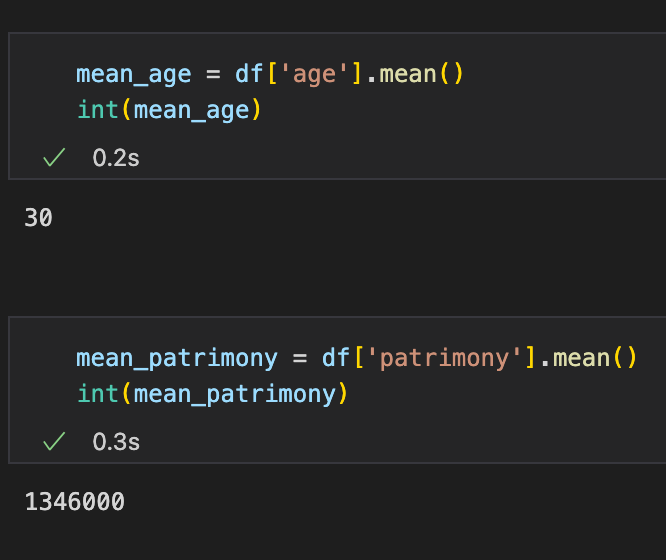
\includegraphics[width=5cm]{../images/illustrations/mean.png}
      \end{figure}
   \end{minipage}
\end{frame}


\begin{frame}\frametitle{Pandas - Median}
   \begin{minipage}{0.58\linewidth}
      \begin{itemize}
         \item Insensitive to extreme values
         \begin{itemize}
            \item Age: good representation
            \item Patrimony: good representation of the majority
         \end{itemize}
      \end{itemize}
      \vspace{.5cm}
      Order values, then:
      $$median = \frac{x_{center_2} - x_{center_1}}{2}$$
      \begin{figure}[H]
         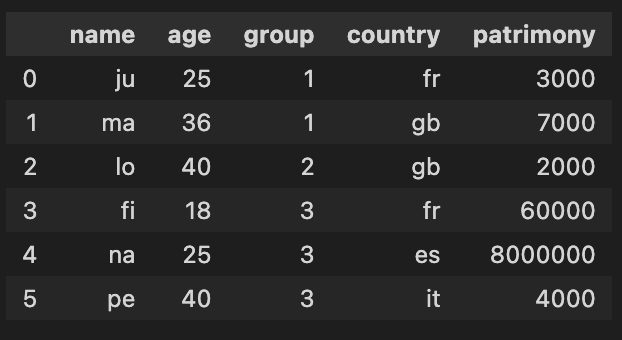
\includegraphics[width=4cm]{../images/illustrations/data_analysis_df_1.png}
      \end{figure}
   \end{minipage}
   \begin{minipage}{0.38\linewidth}
      \begin{figure}[H]
         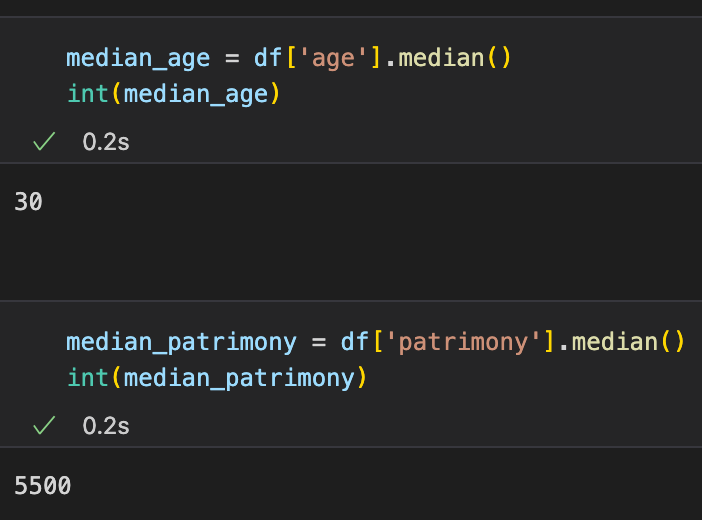
\includegraphics[width=5cm]{../images/illustrations/median.png}
      \end{figure}
   \end{minipage}
\end{frame}



\subsubsection{Dispersion}
%------------------------------------------------------------------------------


\begin{frame}\frametitle{Pandas - Standard Deviation (std)}
   \begin{minipage}{0.58\linewidth}
      \begin{itemize}
         \item Sensible to extreme values
         \item In the unit of the varaible
         \item Interpretable
         \begin{itemize}
            \item Age: good representation
            \item Patrimony: Patrimony: biased, not representative
         \end{itemize}
      \end{itemize}
      \vspace{.5cm}
      $$\overline{x} = mean(values)$$
      $$std = \sqrt{\frac{(x_1-\overline{x}) + ... + (x_n-\overline{x})}{n}}$$
      \begin{figure}[H]
         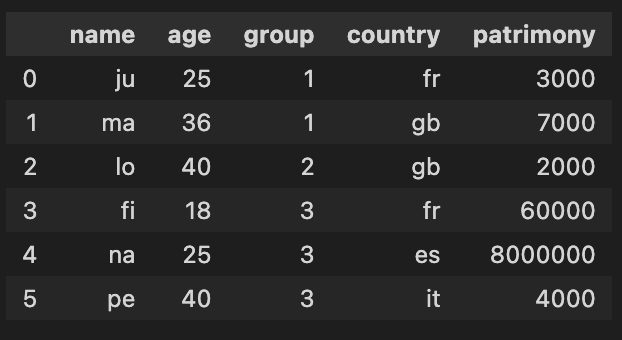
\includegraphics[width=4cm]{../images/illustrations/data_analysis_df_1.png}
      \end{figure}
   \end{minipage}
   \begin{minipage}{0.38\linewidth}
      \begin{figure}[H]
         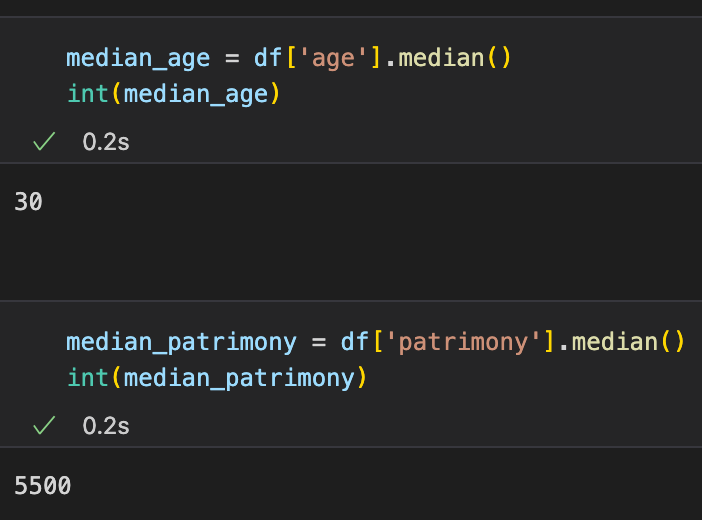
\includegraphics[width=5cm]{../images/illustrations/median.png}
      \end{figure}
   \end{minipage}
\end{frame}


\begin{frame}\frametitle{Pandas - Interquartile Range (iqr)}
   \begin{minipage}{0.58\linewidth}
      \begin{itemize}
         \item Insensitive to extreme values
         \item In the unit of the varaible
         \item Interpretable
         \begin{itemize}
            \item Age: good representation
            \item Patrimony: quite good representation
         \end{itemize}
      \end{itemize}
      \vspace{.5cm}
      $$iqr = 3rd\_quantile - 1st\_quantile$$
      \begin{figure}[H]
         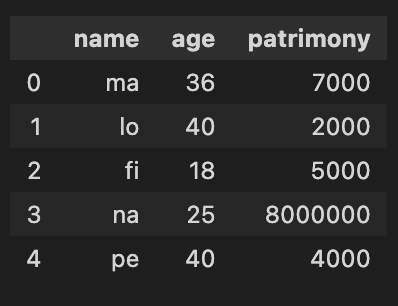
\includegraphics[width=3cm]{../images/illustrations/data_analysis_df_2.png}
      \end{figure}
   \end{minipage}
   \begin{minipage}{0.38\linewidth}
      \begin{figure}[H]
         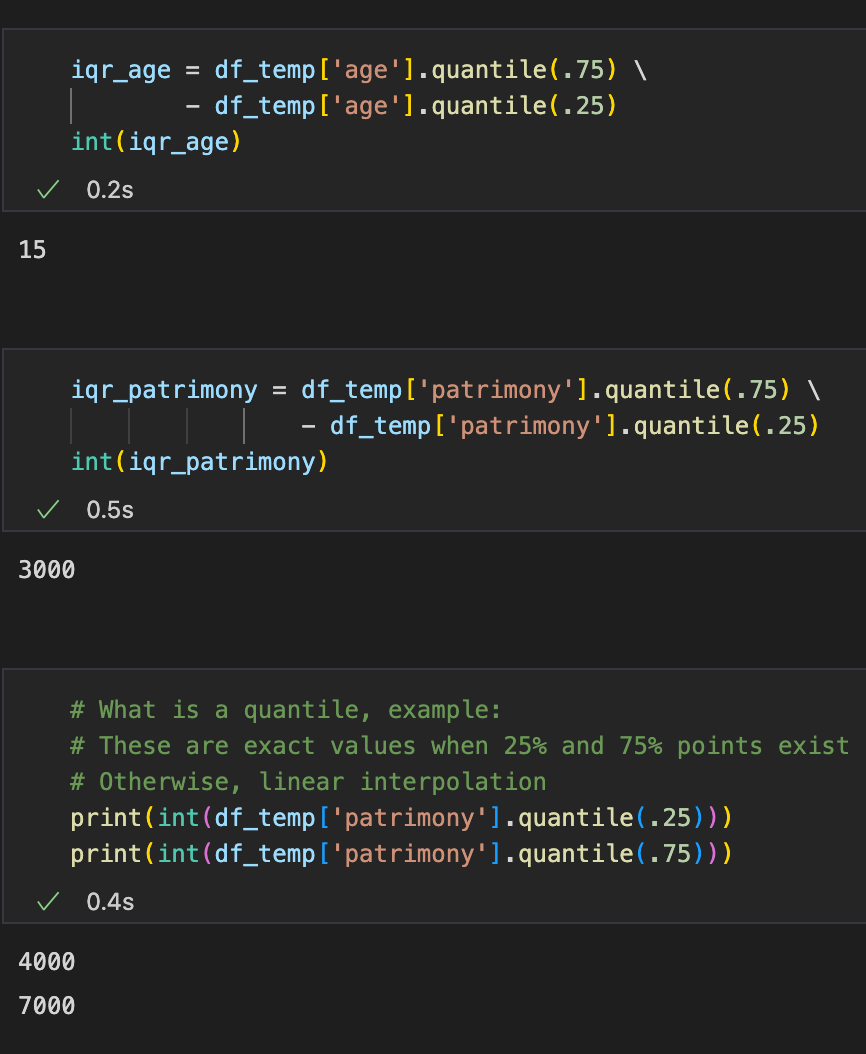
\includegraphics[width=5cm]{../images/illustrations/iqr.png}
      \end{figure}
   \end{minipage}
   \footnote{Quantile values 1st: 25\%, 2nd: 50\%, 3rd: 75\% - after ordering}
\end{frame}



\begin{frame}\frametitle{Pandas - Min Max}
   \begin{minipage}{0.58\linewidth}
      \begin{itemize}
         \item Sensible to extreme values
         \item In the unit of the variable
         \item Interpretable
         \item Easy to compute
         \item Idea of max range
      \end{itemize}
      \vspace{.5cm}
      $$min-max = max(values) - min(values)$$
      \begin{figure}[H]
         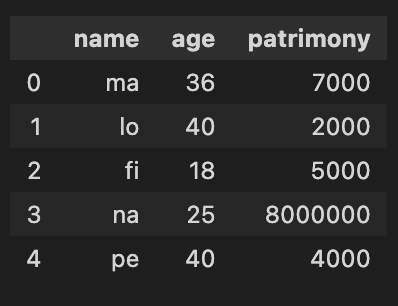
\includegraphics[width=3cm]{../images/illustrations/data_analysis_df_2.png}
      \end{figure}
   \end{minipage}
   \begin{minipage}{0.38\linewidth}
      \begin{figure}[H]
         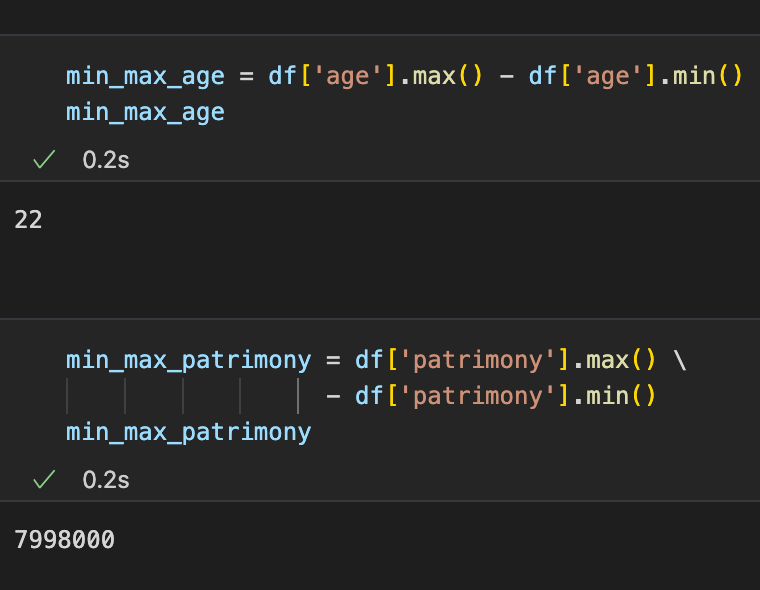
\includegraphics[width=5cm]{../images/illustrations/min_max.png}
      \end{figure}
   \end{minipage}
\end{frame}



%------------------------------------------------------------------------------
\subsection{Data Analysis - Patterns}
%------------------------------------------------------------------------------

\begin{frame}\frametitle{Patterns Analysis}
   \begin{itemize}
      \item Univariate Analysis
      \begin{itemize}
         \item Time Series
         \begin{itemize}
            \item Trend
            \item Seasonality
            \item Auto-correlation
         \end{itemize}
         \item Other quantitative variables
         \item Qualitative variables
      \end{itemize}
      \item Multivariate Analysis (between variables)
      \begin{itemize}
         \item Quantitative variables
         \begin{itemize}
            \item Linear
            \item Non-Linear
         \end{itemize}
         \item Qualitative variables
         %TODO: with ordering
      \end{itemize}
   \end{itemize}
\end{frame}


\subsubsection{Univariate Analysis}
%------------------------------------------------------------------------------

% Time Series
%------------

\begin{frame}\frametitle{Univariate Analysis}
   \begin{minipage}{0.58\linewidth}
      \begin{itemize}
         \item Time Series
         \begin{itemize}
            \item Generate plot using Pandas DataFrame method
         \end{itemize}
      \end{itemize}
      \vspace{.5cm}
      \begin{figure}[H]
         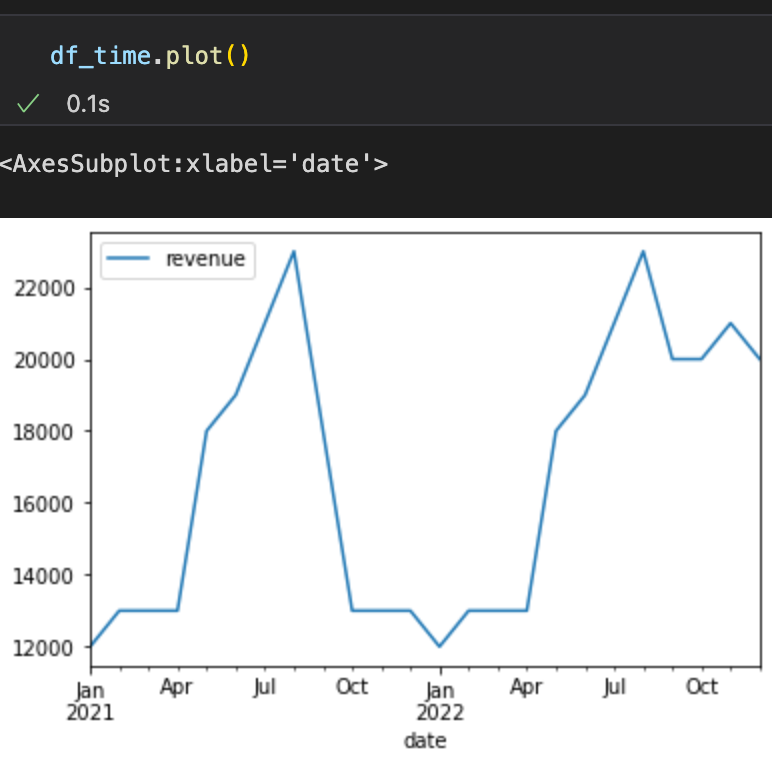
\includegraphics[width=5cm]{../images/illustrations/pattern_graph_time_series_creation.png}
      \end{figure}
   \end{minipage}
   \begin{minipage}{0.38\linewidth}
      \begin{figure}[H]
         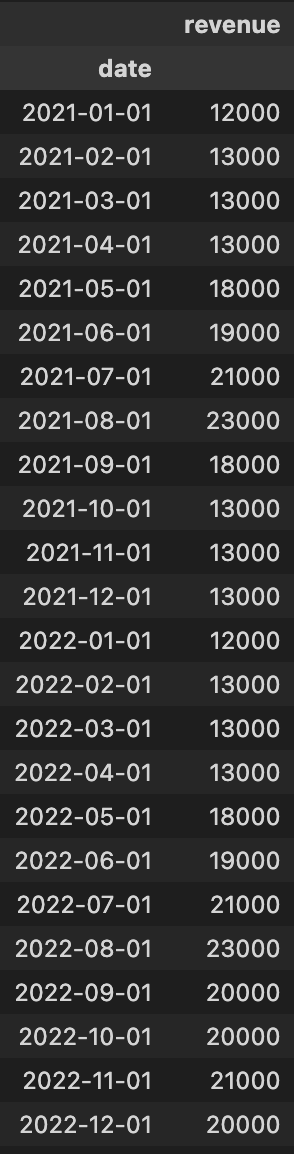
\includegraphics[width=2cm]{../images/illustrations/pattern_df_time_series.png}
      \end{figure}
   \end{minipage}
\end{frame}


\begin{frame}\frametitle{Univariate Analysis}
   \begin{minipage}{0.58\linewidth}
      \begin{itemize}
         \item Time Series
         \begin{itemize}
            \item Compute overall trend
         \end{itemize}
      \end{itemize}
      \vspace{.5cm}
      \begin{figure}[H]
         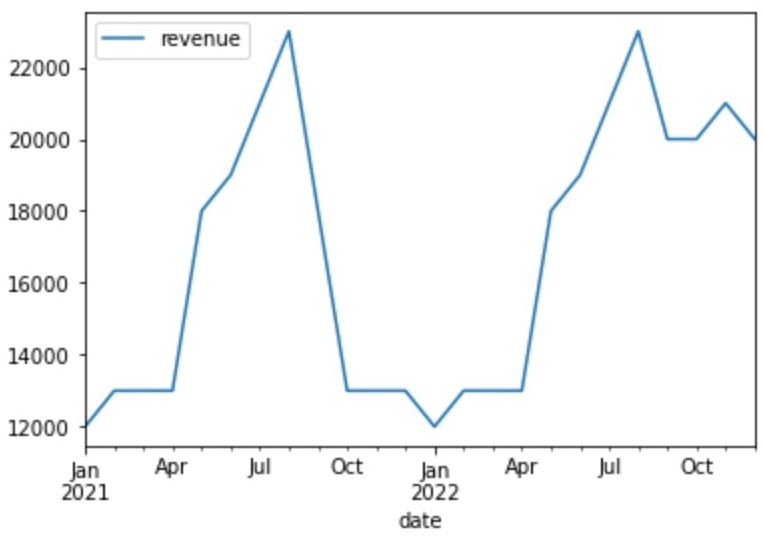
\includegraphics[width=5cm]{../images/illustrations/pattern_graph_time_series.jpg}
      \end{figure}
   \end{minipage}
   \begin{minipage}{0.38\linewidth}
      \begin{figure}[H]
         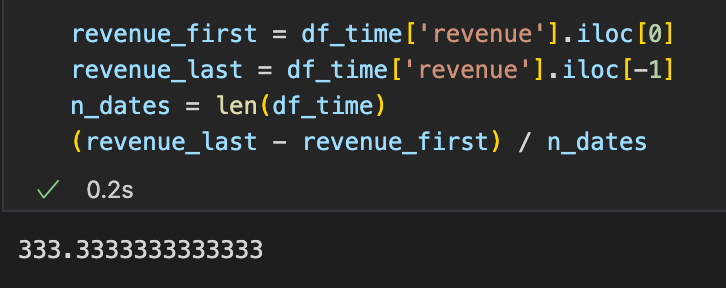
\includegraphics[width=5cm]{../images/illustrations/pattern_compute_trend_overall.png}
      \end{figure}
   \end{minipage}
\end{frame}


\begin{frame}\frametitle{Univariate Analysis}
   \begin{minipage}{0.48\linewidth}
      \begin{itemize}
         \item Time Series
         \begin{itemize}
            \item Compute rolling mean
            \begin{itemize}
               \item Get trend along time
               \item Smoothen curve, easier to read
               \item + info vs overall trend
               \item Delay first dates
            \end{itemize}
         \end{itemize}
      \end{itemize}
      \vspace{.5cm}
      \begin{figure}[H]
         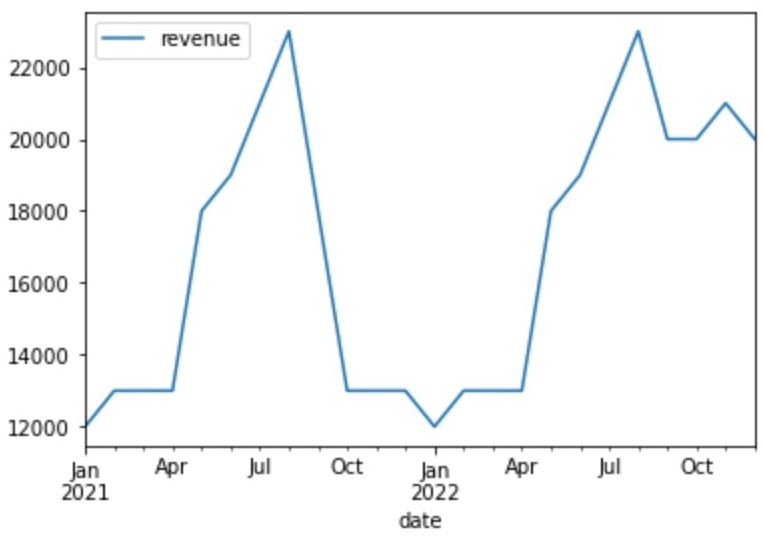
\includegraphics[width=4cm]{../images/illustrations/pattern_graph_time_series.jpg}
      \end{figure}
   \end{minipage}
   \begin{minipage}{0.48\linewidth}
      \begin{figure}[H]
         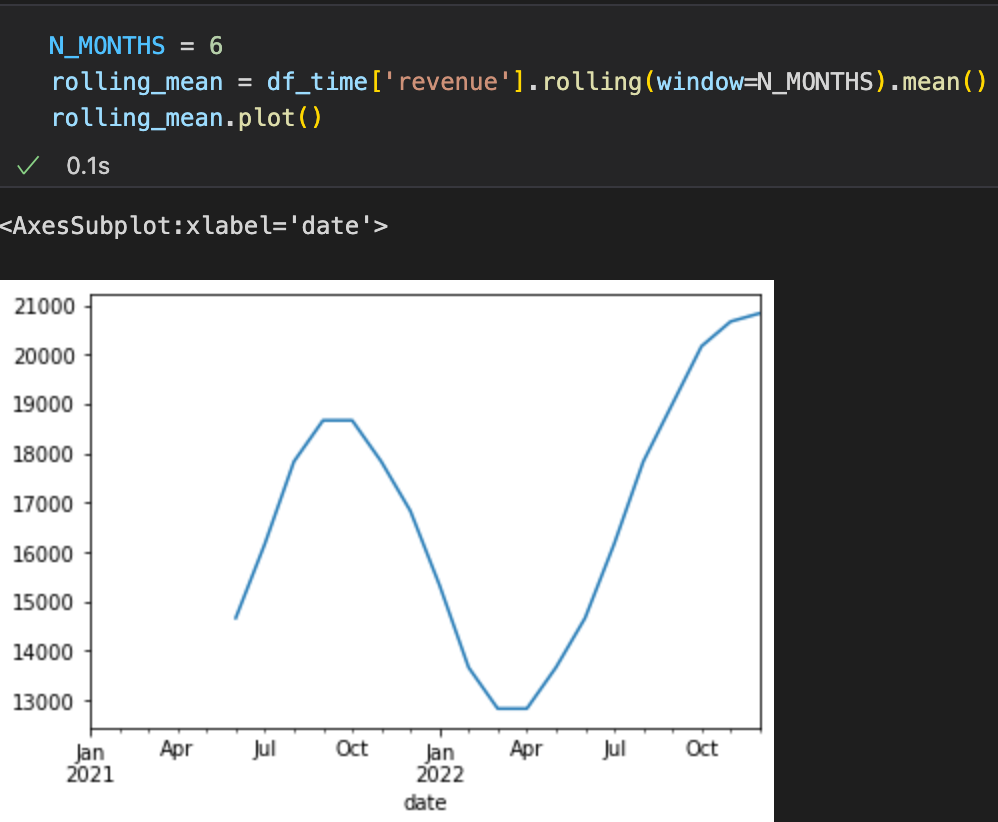
\includegraphics[width=6cm]{../images/illustrations/pattern_graph_time_series_moving_average.png}
      \end{figure}
   \end{minipage}
\end{frame}


\begin{frame}\frametitle{Univariate Analysis}
   \begin{minipage}{0.48\linewidth}
      \begin{itemize}
         \item Time Series
         \begin{itemize}
            \item Autocorrelogram
            \begin{itemize}
               \item Correlation between dates (lags)
            \end{itemize}
         \end{itemize}
      \end{itemize}
      \vspace{.5cm}
      \begin{figure}[H]
         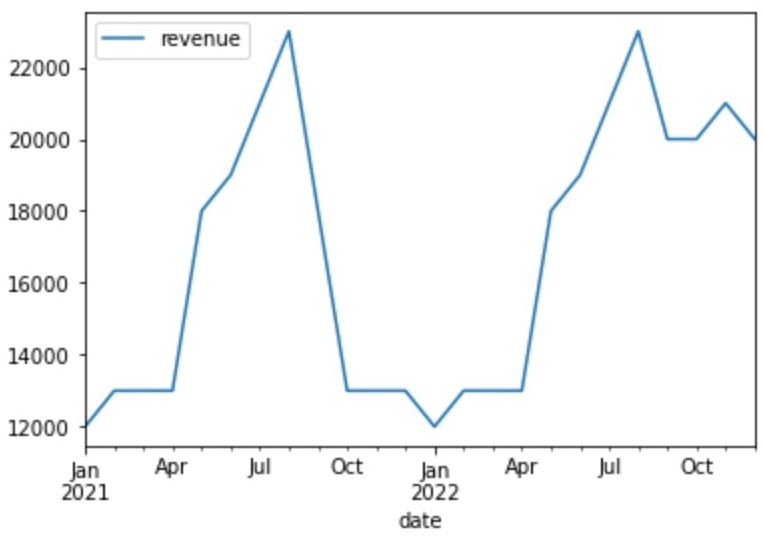
\includegraphics[width=4cm]{../images/illustrations/pattern_graph_time_series.jpg}
      \end{figure}
   \end{minipage}
   \begin{minipage}{0.48\linewidth}
      \begin{figure}[H]
         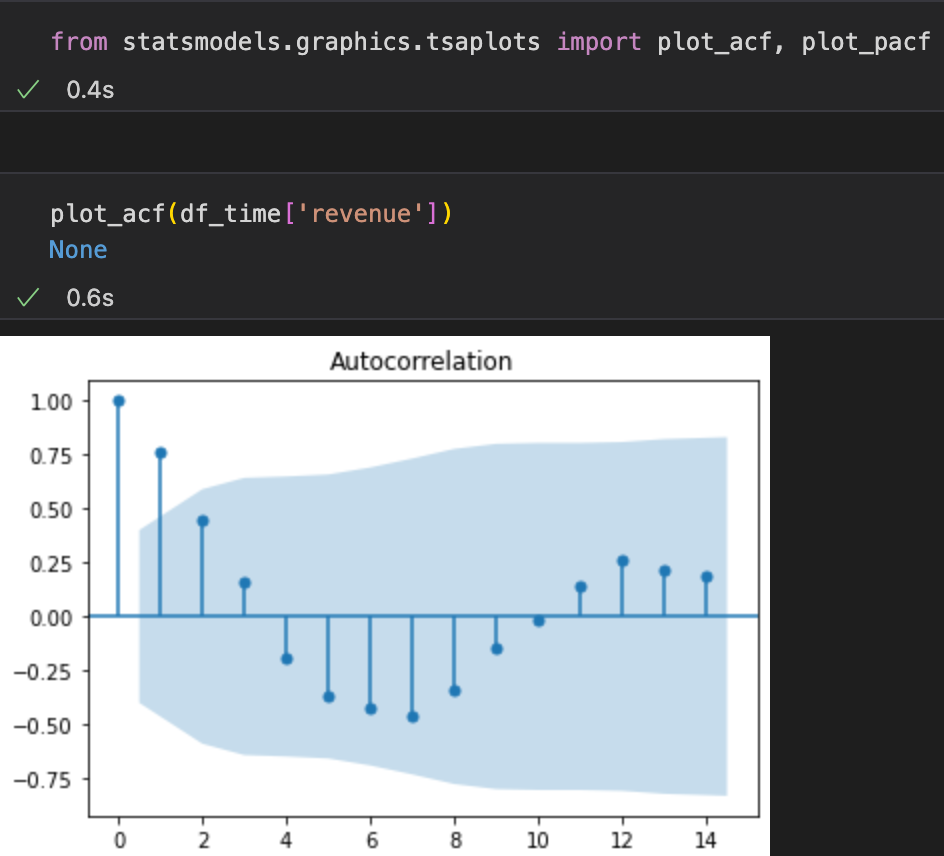
\includegraphics[width=6cm]{../images/illustrations/pattern_graph_autocorrelation.png}
      \end{figure}
   \end{minipage}
\end{frame}



% Other quantitative variables
%-----------------------------


\begin{frame}\frametitle{Univariate Analysis}
   \begin{minipage}{0.48\linewidth}
      \begin{itemize}
         \item Other quantitative variables
         \begin{itemize}
            \item Descriptive statistics
         \end{itemize}
      \end{itemize}
      \vspace{.5cm}
      \begin{figure}[H]
         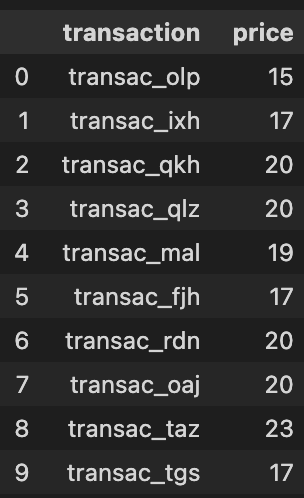
\includegraphics[width=2.2cm]{../images/illustrations/pattern_univariate_quantitative_df.png}
      \end{figure}
   \end{minipage}
   \begin{minipage}{0.48\linewidth}
      \begin{figure}[H]
         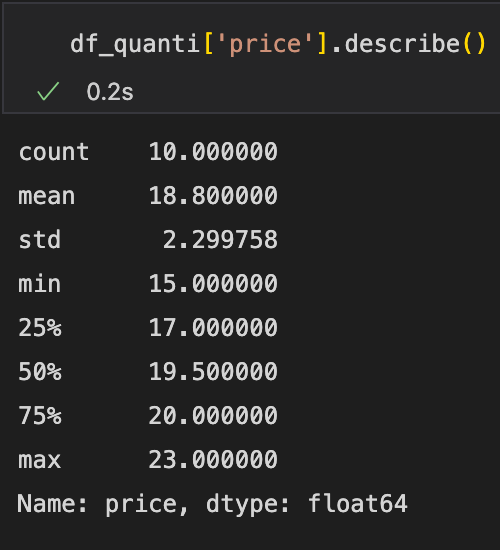
\includegraphics[width=3.5cm]{../images/illustrations/pattern_univariate_quantitative_describe.png}
      \end{figure}
   \end{minipage}
\end{frame}



\begin{frame}\frametitle{Univariate Analysis}
   \begin{minipage}{0.48\linewidth}
      \begin{itemize}
         \item Other quantitative variables
         \begin{itemize}
            \item Histogram
            \begin{itemize}
               \item Overview
               \item Extreme values
               \item All information
            \end{itemize}
         \end{itemize}
      \end{itemize}
      \vspace{.5cm}
      \begin{figure}[H]
         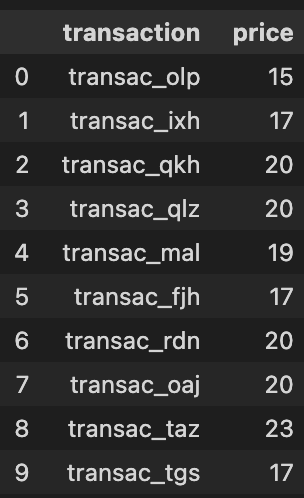
\includegraphics[width=2.2cm]{../images/illustrations/pattern_univariate_quantitative_df.png}
      \end{figure}
   \end{minipage}
   \begin{minipage}{0.48\linewidth}
      \begin{figure}[H]
         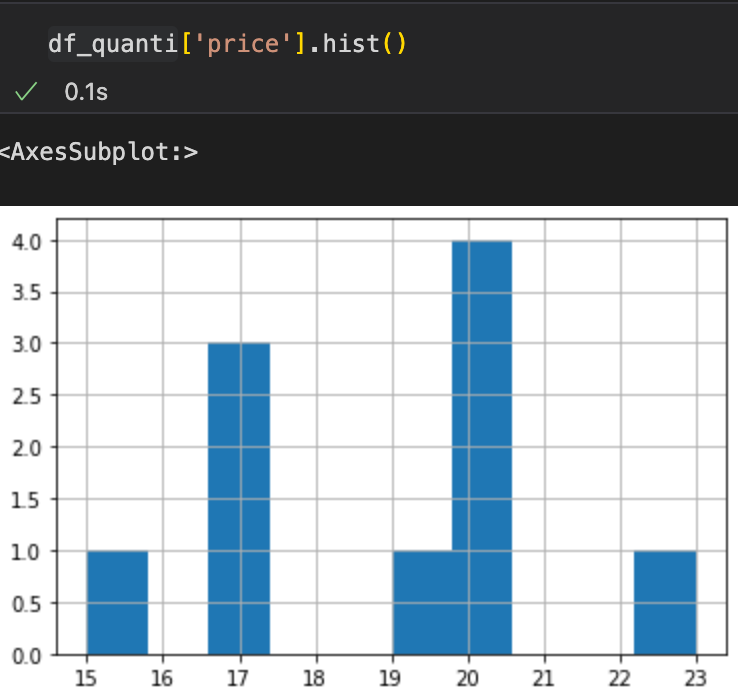
\includegraphics[width=5cm]{../images/illustrations/pattern_univariate_quantitative_hist.png}
      \end{figure}
   \end{minipage}
\end{frame}



\begin{frame}\frametitle{Univariate Analysis}
   \begin{minipage}{0.48\linewidth}
      \begin{itemize}
         \item Other quantitative variables
         \begin{itemize}
            \item Boxplot
            \begin{itemize}
               \item Overview
               \item Extreme values
               \item Contracted information
               \item Quartiles
               \item Outliers (seaborn)
            \end{itemize}
         \end{itemize}
      \end{itemize}
      \vspace{.5cm}
      \begin{figure}[H]
         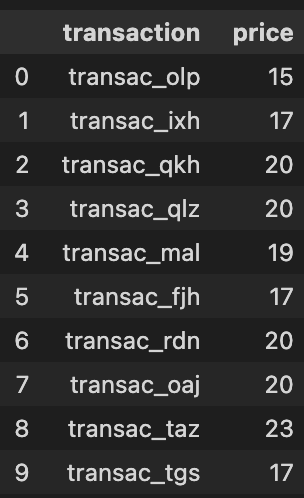
\includegraphics[width=2.2cm]{../images/illustrations/pattern_univariate_quantitative_df.png}
      \end{figure}
   \end{minipage}
   \begin{minipage}{0.48\linewidth}
      \begin{figure}[H]
         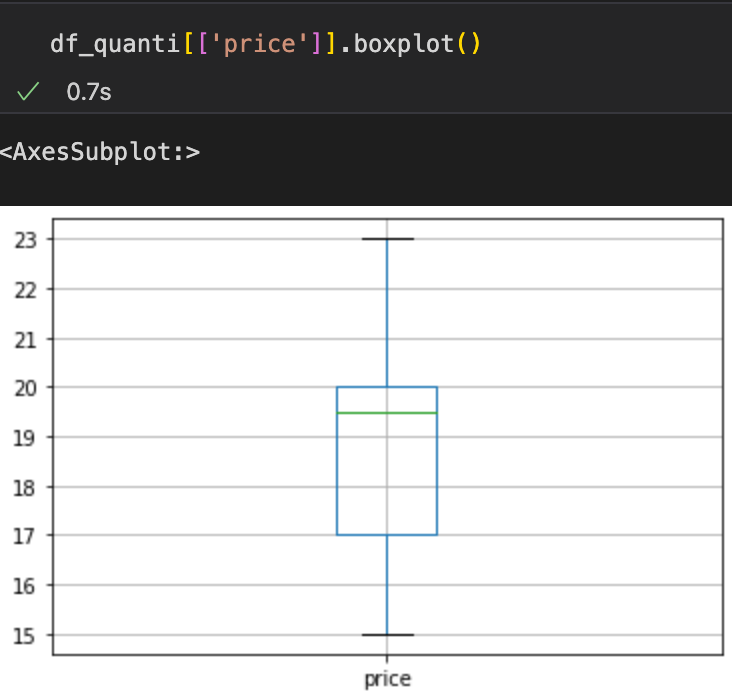
\includegraphics[width=5cm]{../images/illustrations/pattern_univariate_quantitative_boxplot.png}
      \end{figure}
   \end{minipage}
\end{frame}


% Qualitative variables
%----------------------

\begin{frame}\frametitle{Univariate Analysis}
   \begin{minipage}{0.48\linewidth}
      \begin{itemize}
         \item Qualitative variables
         \begin{itemize}
            \item Information on categories
         \end{itemize}
      \end{itemize}
      \vspace{.5cm}
      \begin{figure}[H]
         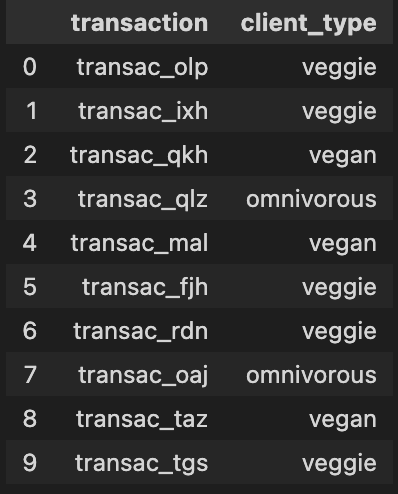
\includegraphics[width=3cm]{../images/illustrations/pattern_univariate_qualitative_df.png}
      \end{figure}
   \end{minipage}
   \begin{minipage}{0.48\linewidth}
      \begin{figure}[H]
         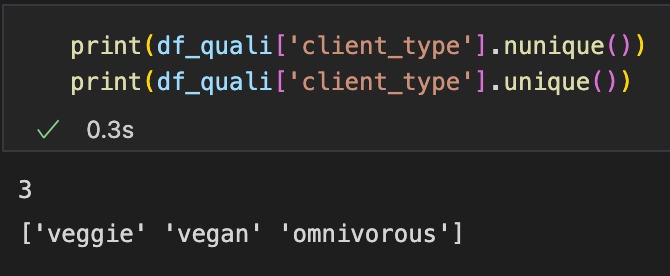
\includegraphics[width=5cm]{../images/illustrations/pattern_univariate_qualitative_uniques.png}
      \end{figure}
      \begin{figure}[H]
         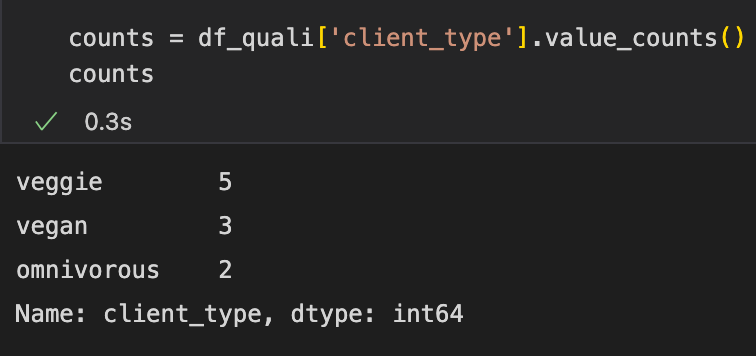
\includegraphics[width=5cm]{../images/illustrations/pattern_univariate_qualitative_counts.png}
      \end{figure}
   \end{minipage}
\end{frame}


\begin{frame}\frametitle{Univariate Analysis}
   \begin{minipage}{0.48\linewidth}
      \begin{itemize}
         \item Qualitative variables
         \begin{itemize}
            \item Bar plot
            \begin{itemize}
               \item Overview
               \item Ordinal variables: (small, medium, large companies)
            \end{itemize}
         \end{itemize}
      \end{itemize}
      \vspace{.5cm}
      \begin{figure}[H]
         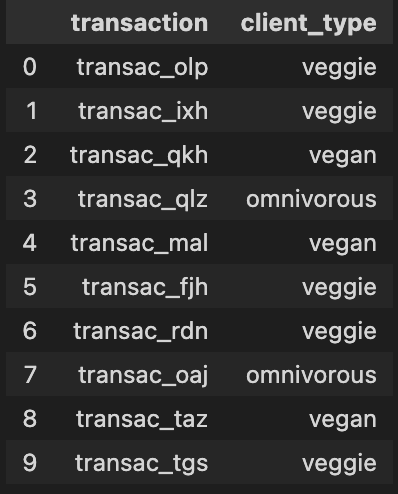
\includegraphics[width=3cm]{../images/illustrations/pattern_univariate_qualitative_df.png}
      \end{figure}
   \end{minipage}
   \begin{minipage}{0.48\linewidth}
      \begin{figure}[H]
         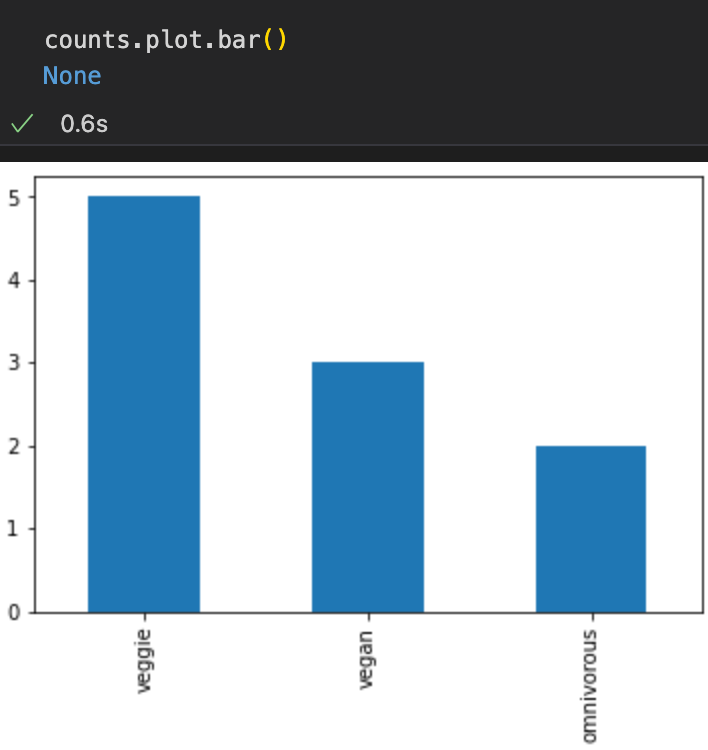
\includegraphics[width=5cm]{../images/illustrations/pattern_univariate_qualitative_bars.png}
      \end{figure}
   \end{minipage}
\end{frame}



\subsubsection{Multivariate Analysis}
%------------------------------------------------------------------------------
% TODO: add axes names to each graph (everywhere)


% Linear data
%------------


\begin{frame}\frametitle{Multivariate Analysis}
   \begin{minipage}{0.48\linewidth}
      \begin{itemize}
         \item Quantitative variables\\
               with linear relation
         \begin{itemize}
            \item Scatter plot
            \item Linear regression
            \item Relation / link
         \end{itemize}
      \end{itemize}
      \vspace{.5cm}
      \begin{figure}[H]
         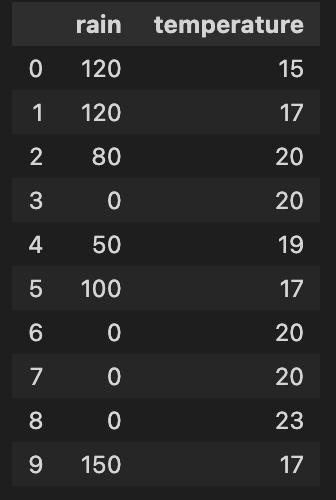
\includegraphics[width=2.5cm]{../images/illustrations/pattern_multivariate_quantitative_df.png}
      \end{figure}
   \end{minipage}
   \begin{minipage}{0.48\linewidth}
      \begin{figure}[H]
         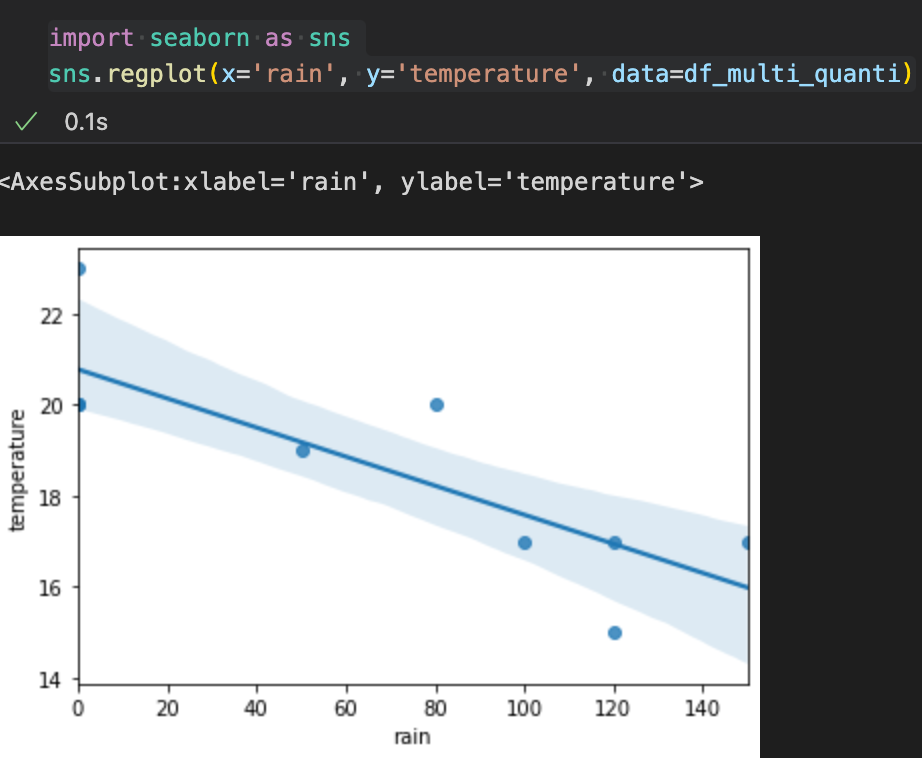
\includegraphics[width=6cm]{../images/illustrations/pattern_multivariate_quantitative_scatter.png}
      \end{figure}
   \end{minipage}
\end{frame}



\begin{frame}\frametitle{Multivariate Analysis}
   \begin{minipage}{0.48\linewidth}
      \begin{itemize}
         \item Quantitative variables\\
               with linear relation
         \begin{itemize}
            \item Bar plot raw data
            \item More interesting when Time Series (not here)
         \end{itemize}
      \end{itemize}
      \vspace{.5cm}
      \begin{figure}[H]
         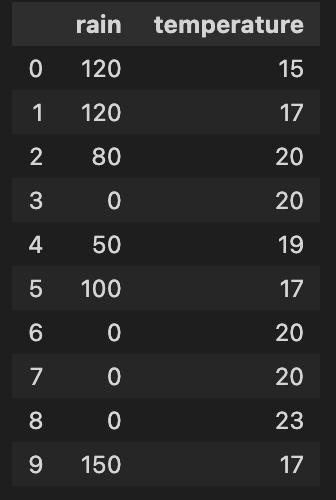
\includegraphics[width=2.5cm]{../images/illustrations/pattern_multivariate_quantitative_df.png}
      \end{figure}
   \end{minipage}
   \begin{minipage}{0.48\linewidth}
      \begin{figure}[H]
         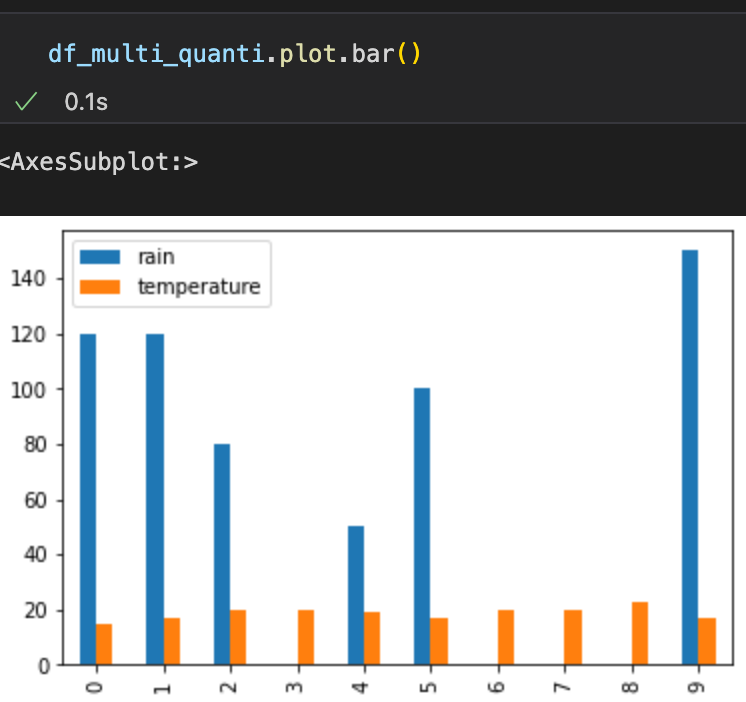
\includegraphics[width=5cm]{../images/illustrations/pattern_multivariate_quantitative_bar_raw_data.png}
      \end{figure}
   \end{minipage}
\end{frame}


\begin{frame}\frametitle{Multivariate Analysis}
   \begin{minipage}{0.48\linewidth}
      \begin{itemize}
         \item Quantitative variables\\
               with linear relation
         \begin{itemize}
            \item Correlation matrix
            \item Pearson correlation (linear)
            \item Symetric matrix
         \end{itemize}
      \end{itemize}
      \vspace{.5cm}
      \begin{figure}[H]
         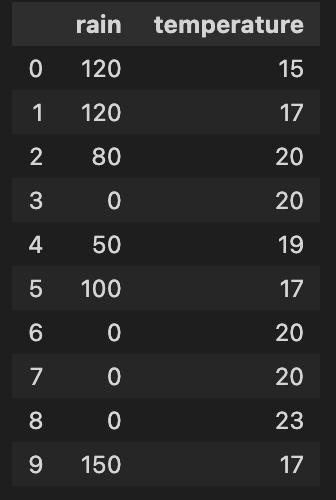
\includegraphics[width=2.5cm]{../images/illustrations/pattern_multivariate_quantitative_df.png}
      \end{figure}
   \end{minipage}
   \begin{minipage}{0.48\linewidth}
      \begin{figure}[H]
         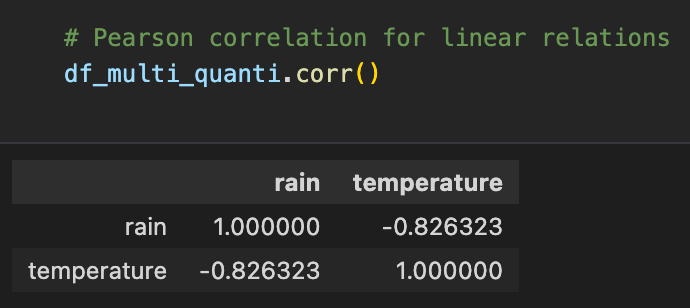
\includegraphics[width=5cm]{../images/illustrations/pattern_multivariate_quantitative_corr.png}
      \end{figure}
   \end{minipage}
\end{frame}


\begin{frame}\frametitle{Multivariate Analysis}
   \begin{minipage}{0.48\linewidth}
      \begin{itemize}
         \item Quantitative variables\\
               with linear relation
         \begin{itemize}
            \item Pairplot: Histograms and scatter plots
            \item Very useful for +3 variables
         \end{itemize}
      \end{itemize}
      \vspace{.5cm}
      \begin{figure}[H]
         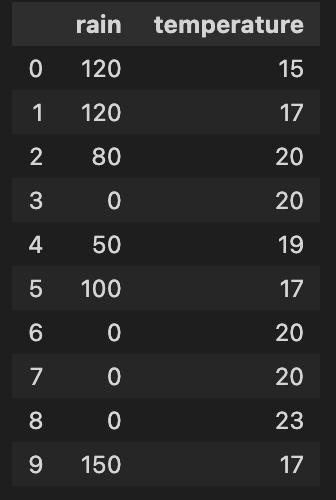
\includegraphics[width=2.5cm]{../images/illustrations/pattern_multivariate_quantitative_df.png}
      \end{figure}
   \end{minipage}
   \begin{minipage}{0.48\linewidth}
      \begin{figure}[H]
         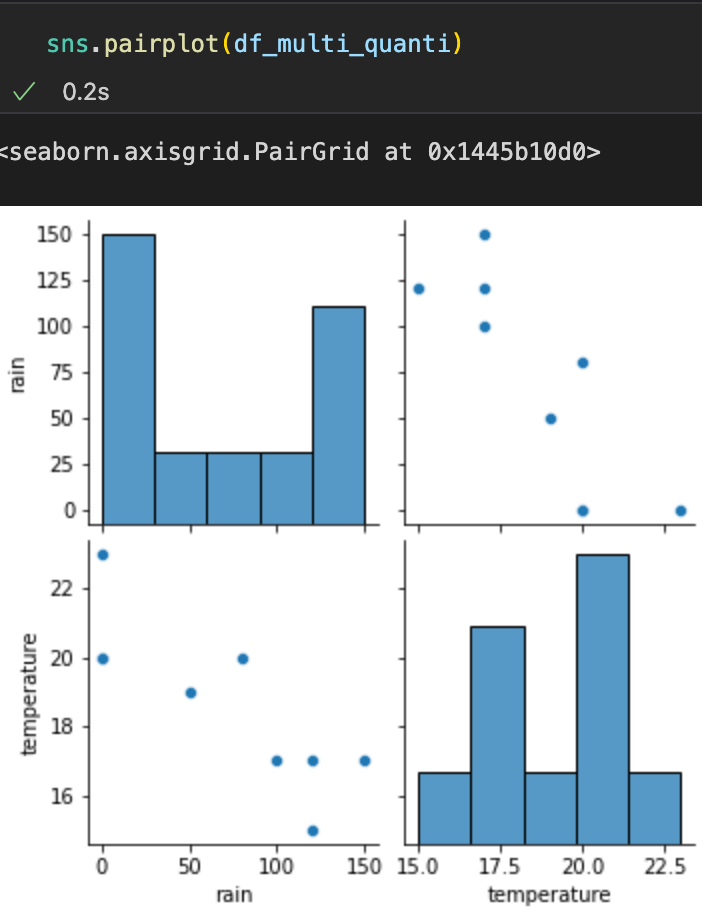
\includegraphics[width=5cm]{../images/illustrations/pattern_multivariate_quantitative_pairplot.png}
      \end{figure}
   \end{minipage}
\end{frame}


\begin{frame}\frametitle{Multivariate Analysis}
   \begin{minipage}{0.48\linewidth}
      \begin{itemize}
         \item Quantitative variables\\
               with linear relation
         \begin{itemize}
            \item Groupby
            \item Aggregation functions: mean, max, std, etc.
            \item Groups: type of clients, of investments, etc.
            \item Less information, more lisibility
         \end{itemize}
      \end{itemize}
      \begin{figure}[H]
         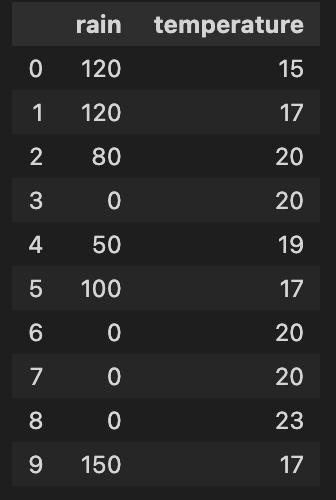
\includegraphics[width=2.5cm]{../images/illustrations/pattern_multivariate_quantitative_df.png}
      \end{figure}
   \end{minipage}
   \begin{minipage}{0.48\linewidth}
      \begin{figure}[H]
         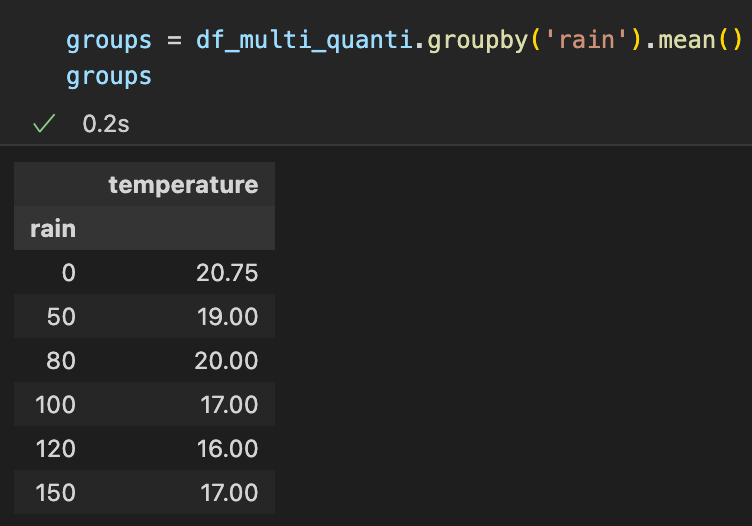
\includegraphics[width=5cm]{../images/illustrations/pattern_multivariate_quantitative_groupby.png}
      \end{figure}
   \end{minipage}
\end{frame}


\begin{frame}\frametitle{Multivariate Analysis}
   \begin{minipage}{0.48\linewidth}
      \begin{itemize}
         \item Quantitative variables\\
               with linear relation
         \begin{itemize}
            \item Bar plot
            \item Here based on grouped data
            \item Complementary to raw data bar plot
         \end{itemize}
      \end{itemize}
      \begin{figure}[H]
         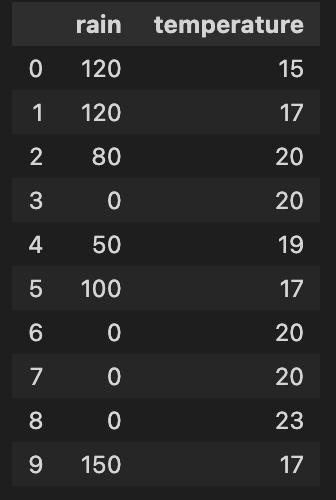
\includegraphics[width=2.5cm]{../images/illustrations/pattern_multivariate_quantitative_df.png}
      \end{figure}
   \end{minipage}
   \begin{minipage}{0.48\linewidth}
      \begin{figure}[H]
         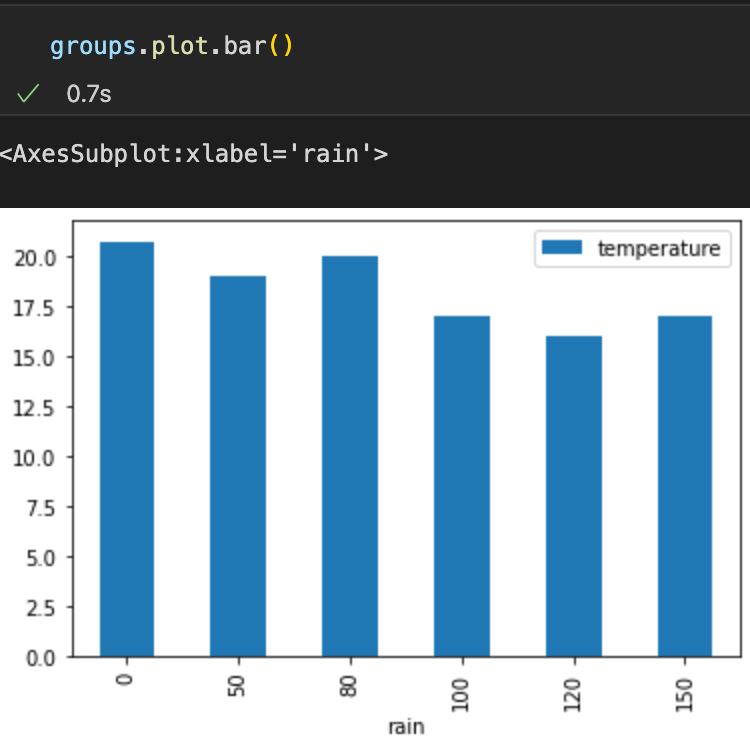
\includegraphics[width=5cm]{../images/illustrations/pattern_multivariate_quantitative_bar_grouped.png}
      \end{figure}
   \end{minipage}
\end{frame}


% Non-linear data
%----------------


\begin{frame}\frametitle{Multivariate Analysis}
   \begin{minipage}{0.48\linewidth}
      \begin{itemize}
         \item Quantitative variables\\
               with non-linear relation
         \begin{itemize}
            \item Scatter plot
            \item Linear regression misleading
         \end{itemize}
      \end{itemize}
      \vspace{.5cm}
      \begin{figure}[H]
         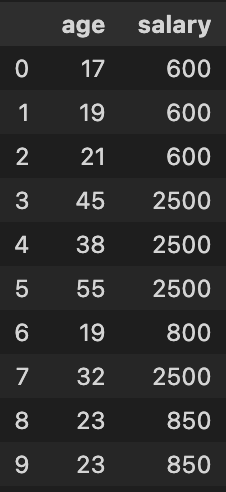
\includegraphics[width=1.8cm]{../images/illustrations/pattern_multivariate_quantitative_non_linear_df.png}
      \end{figure}
   \end{minipage}
   \begin{minipage}{0.48\linewidth}
      \begin{figure}[H]
         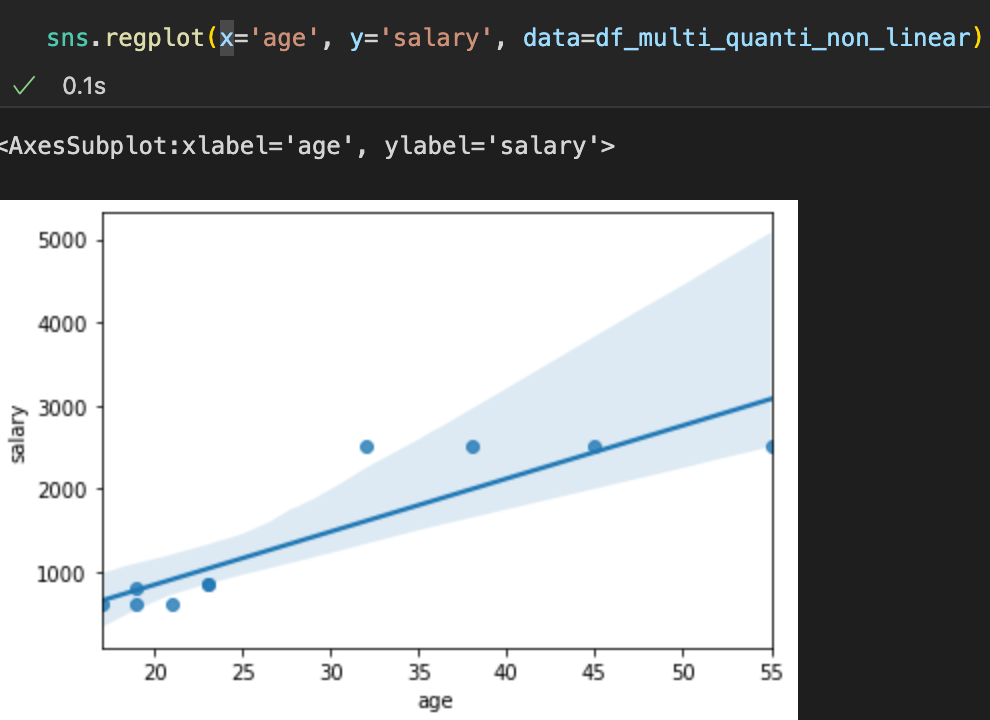
\includegraphics[width=6cm]{../images/illustrations/pattern_multivariate_quantitative_non_linear_scatter.png}
      \end{figure}
   \end{minipage}
\end{frame}


\begin{frame}\frametitle{Multivariate Analysis}
   \begin{minipage}{0.48\linewidth}
      \begin{itemize}
         \item Quantitative variables\\
               with non-linear relation
         \begin{itemize}
            \item Correlation matrix
            \item Pearson correlation (linear) also misleading
         \end{itemize}
      \end{itemize}
      \vspace{.5cm}
      \begin{figure}[H]
         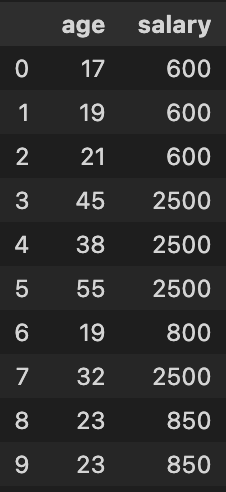
\includegraphics[width=1.8cm]{../images/illustrations/pattern_multivariate_quantitative_non_linear_df.png}
      \end{figure}
   \end{minipage}
   \begin{minipage}{0.48\linewidth}
      \begin{figure}[H]
         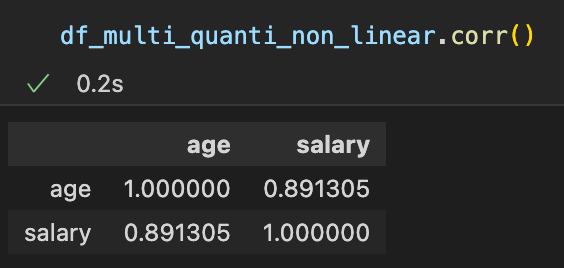
\includegraphics[width=4.2cm]{../images/illustrations/pattern_multivariate_quantitative_non_linear_corr_pearson.png}
      \end{figure}
   \end{minipage}
\end{frame}

\begin{frame}\frametitle{Multivariate Analysis}
   \begin{minipage}{0.48\linewidth}
      \begin{itemize}
         \item Quantitative variables\\
               with non-linear relation
         \begin{itemize}
            \item Correlation matrix
            \item Spearman correlation (non-linear) instead
            \item Rank based correlation
         \end{itemize}
      \end{itemize}
      \vspace{.5cm}
      \begin{figure}[H]
         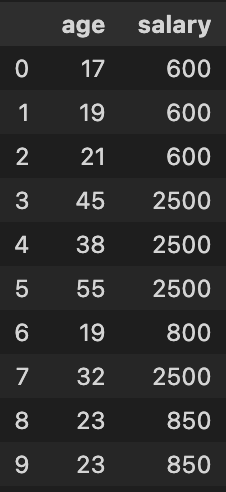
\includegraphics[width=1.8cm]{../images/illustrations/pattern_multivariate_quantitative_non_linear_df.png}
      \end{figure}
   \end{minipage}
   \begin{minipage}{0.5\linewidth}
      \begin{figure}[H]
         \includegraphics[width=6.6cm]{../images/illustrations/pattern_multivariate_quantitative_non_linear_corr_spearman.png}
      \end{figure}
   \end{minipage}
\end{frame}


\begin{frame}\frametitle{Multivariate Analysis}
   \begin{minipage}{0.48\linewidth}
      \begin{itemize}
         \item Quantitative variables\\
               with non-linear relation
         \begin{itemize}
            \item Pairplot
            \item Different regims well separated?
         \end{itemize}
      \end{itemize}
      \vspace{.5cm}
      \begin{figure}[H]
         \includegraphics[width=1.8cm]{../images/illustrations/pattern_multivariate_quantitative_non_linear_df.png}
      \end{figure}
   \end{minipage}
   \begin{minipage}{0.48\linewidth}
      \begin{figure}[H]
         \includegraphics[width=5cm]{../images/illustrations/pattern_multivariate_quantitative_non_linear_pairplot.png}
      \end{figure}
   \end{minipage}
\end{frame}


\begin{frame}\frametitle{Multivariate Analysis}
   \begin{minipage}{0.48\linewidth}
      \begin{itemize}
         \item Quantitative variables\\
               with non-linear relation
         \begin{itemize}
            \item Analyse regimes relations separatly
         \end{itemize}
      \end{itemize}
      \begin{figure}[H]
         \includegraphics[width=1.8cm]{../images/illustrations/pattern_multivariate_quantitative_non_linear_df.png}
      \end{figure}
   \end{minipage}
   \begin{minipage}{0.48\linewidth}
      \begin{figure}[H]
         \includegraphics[width=5.5cm]{../images/illustrations/pattern_multivariate_quantitative_non_linear_regressions.png}
      \end{figure}
   \end{minipage}
\end{frame}


\begin{frame}\frametitle{Multivariate Analysis}
   \begin{minipage}{0.48\linewidth}
      \begin{itemize}
         \item Quantitative variables\\
               with non-linear relation
         \begin{itemize}
            \item Analyse regimes correlations separatly
         \end{itemize}
      \end{itemize}
      \begin{figure}[H]
         \includegraphics[width=1.8cm]{../images/illustrations/pattern_multivariate_quantitative_non_linear_df.png}
      \end{figure}
   \end{minipage}
   \begin{minipage}{0.48\linewidth}
      \begin{figure}[H]
         \includegraphics[width=3cm]{../images/illustrations/pattern_multivariate_quantitative_non_linear_corr_pearson_split.png}
      \end{figure}
   \end{minipage}
\end{frame}

% here
%------------------------------------------------------------------------------
\subsection{Statistical Tools}
%------------------------------------------------------------------------------


\begin{frame}\frametitle{Correlation}
   \begin{itemize}
      \item Move repetitively in conjunction
      \item Methods
      \begin{itemize}
         \item Pearson
         \item Spearman (Rank)
      \end{itemize}
      \item Spurious correlation (ice cream, Eiffel Tower)
   \end{itemize}
\end{frame}



\subsubsection{Statistical Laws}

\begin{frame}\frametitle{Statistical Laws}
   \begin{itemize}
      \item Normal Law / Gauss Curve
      \begin{itemize}
         \item Totally resumed by mean and variance
         \item Constant mean (0 if centered) and variance (1 if reduced)
         \item Uncorrelated individuals
         \item Symetric (Skewness=0)
         \item Precise bell shape (Kurtosis=3)
      \end{itemize}

      \item Power Laws: multiplicative growth
      % TODO: insert graph examples of both distributions
      \item Examples:
      \begin{itemize}
         \item Normal: human age, size, weight, grades
         \item Power: lakes size, wealth
      \end{itemize}
   \end{itemize}
\end{frame}


\subsubsection{Statistical Tests}

\begin{frame}\frametitle{Statistical Tests}
   \begin{itemize}
      \item Intention: prevent sampling error
      \item Hypothesis (Normal Law)
      \item Examples:
      \begin{itemize}
         \item Normality test
         \item ANOVA
         \item Pearson's r
         \item Chi square
      \end{itemize}
         % TODO: review https://www.scribbr.com/statistics/statistical-tests/
   \end{itemize}
\end{frame}



\end{document}